\problemname{\problemyamlname}

\illustration{0.3}{image.jpg}{
    CC BY-SA 4.0 par commercialart sur \href{https://www.vecteezy.com/vector-art/190747-ride-rollercoaster}{vecteezy}
}

Vous êtes invité par vos amis au célèbre parc d'attractions \textit{KARWa land}. Bien que vous soyez un peu craintif vis-à-vis des attractions à grande vitesse depuis un accident d'enfance où vous avez chuté de 100 mètres, vous décidez de les accompagner pour ne pas les décevoir. Votre objectif est de profiter au maximum des attractions tout en évitant celles dont la vitesse est strictement supérieure à $a$.

Heureusement, le site Web du parc répertorie les attractions ainsi que la hauteur des rails. Chaque segment de rail est défini par deux points, et la vitesse dans ce segment est la différence de hauteur entre ces deux points. Bien sûr, ici on s'intéresse à la vitesse lorsque l'on descend étant donné que c'est à ce moment-là où l'on a le plus de sensations fortes.

Vous souhaitez déterminer combien d'attractions vous pouvez faire.

\begin{figure}[h]
    \centering
    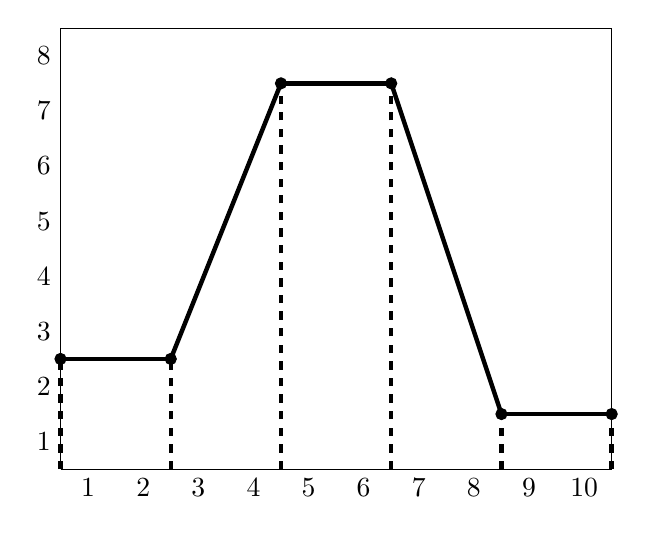
\begin{tikzpicture}[scale=0.70]
      \draw (0,0) -- (10,0) -- (10,8) -- (0,8) -- (0,0);
      \draw[ultra thick] (0,2) -- (2, 2);
      \node at (0, 2) {\pgfuseplotmark{*}};
      \node at (2,2) {\pgfuseplotmark{*}};


      \draw[ultra thick] (2, 2) -- (4, 7);
      \node at (4,7) {\pgfuseplotmark{*}};

      \draw[ultra thick](4,7) -- (6, 7);
      \node at (6,7) {\pgfuseplotmark{*}};

      \draw[ultra thick](6, 7) -- (8, 1);
      \node at (8, 1) {\pgfuseplotmark{*}};

      \draw[ultra thick](8,1) -- (10, 1);
      \node at (10, 1) {\pgfuseplotmark{*}};
    
        % On génère la grille
        \foreach \x in {1, ..., 10} {%
          % Bottom
          \node[anchor=north] at (\x-0.5,0) {\x};
        }
        %
        \foreach \y in {1, ..., 8} {%
        % Left
        \node[anchor=east] at (0,\y-0.5) {\y};
        }

        \draw[ultra thick, dashed] (0, 0) -- (0, 2);
        \draw[ultra thick, dashed] (2, 0) -- (2, 2);
        \draw[ultra thick, dashed] (4, 0) -- (4, 7);
        \draw[ultra thick, dashed] (6, 0) -- (6, 7);
        \draw[ultra thick, dashed] (8, 0) -- (8, 1);
        \draw[ultra thick, dashed] (10, 0) -- (10, 1);
    \end{tikzpicture}
    \caption{Illustration de l'exemple 1}
\end{figure}

\begin{Input}
    L'entrée consiste en :
    \begin{itemize}
        \item une ligne contenant deux entiers $n$ et $a$ ($0 \leq n \leq 1000$, $0 \leq a \leq 6 \cdot 10^6$), représentant respectivement le nombre d'attractions dans le parc et la vitesse maximale que vous pouvez supporter,
        \item $n$ lignes, chacune contenant une chaîne de caractères $s_i$ ($1 \leq |s_i| \leq 10$) et un entier $m_i$ $(2 \leq m_i \leq 1000)$, représentant le nom de l'attraction et le nombre de sommets dans l'attraction, suivis de $m_i$ entiers $x_{i,j}$ ($0 \leq x_{i,j} \leq 10^6$) représentant la hauteur de chaque sommet.
    \end{itemize}
\end{Input}

\begin{Output}
    Sortez un entier $k$ représentant le nombre d'attractions que vous pouvez faire, suivi de $k$ chaînes de caractères représentant le nom de chaque attraction que vous pouvez faire.
\end{Output}
